\documentclass[12pt, twoside]{article}
\usepackage[letterpaper, margin=1in, headsep=0.5in]{geometry}
\usepackage[english]{babel}
\usepackage[utf8]{inputenc}
\usepackage{amsmath}
\usepackage{amsfonts}
\usepackage{amssymb}
\usepackage{tikz}
\usetikzlibrary{quotes, angles}
\usepackage{graphicx}
\usepackage{enumitem}
\usepackage{multicol}

\newif\ifmeta
\metatrue %print standards and topics tags

\title{Regents Geometry}
\author{Chris Huson}
\date{January 2022}

\usepackage{fancyhdr}
\pagestyle{fancy}
\fancyhf{}
\renewcommand{\headrulewidth}{0pt} % disable the underline of the header
\raggedbottom

\fancyhead[LE]{\thepage}
\fancyhead[RO]{\thepage \\ Name: \hspace{4cm} \,\\}
\fancyhead[LO]{BECA / Dr. Huson / Geometry 7 Similarity}

\begin{document}

\subsubsection*{7.4 Prequiz: Dilations and scale \hfill CCSS.HSG.SRT.B.5}
\begin{enumerate}
\begin{multicols}{2}
[\item A dilation maps $\triangle ABC \rightarrow \triangle DEF$, with $AB=10$, $BC=12$, $AC=5$, and $DF=6$.] \vspace{0.5cm}
  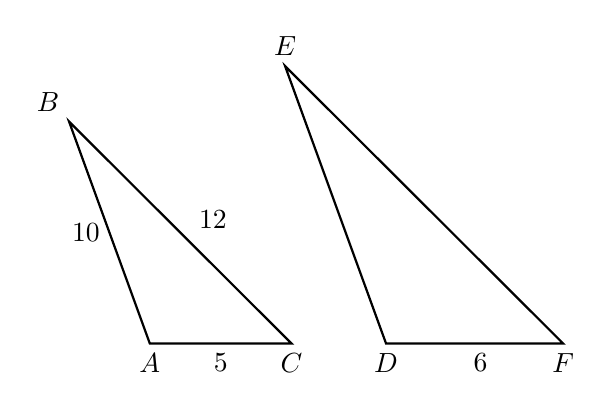
\begin{tikzpicture}[scale=1.2]
    \coordinate [label=above left:$B$](A) at (110:2.5);
    \coordinate [label=below:$A$](B) at (0, 0);
    \coordinate [label=below:$C$](C) at (0:1.5);
    \draw [thick] (A)--(B)--(C)--cycle;
    \draw [thick, xshift=2.5cm, yshift=0cm, scale=1.25, rotate=0] (110:2.5) node[above]{$E$}--
    (0,0) node[below]{$D$}--
    (0:1.5) node[below]{$F$}--cycle;
    \node at (110:1.25)[left]{$10$};
    \node at (55:1.6)[left]{$12$};
    \node at (0:0.75)[below]{$5$};
    \node at (0:3.5)[below]{$6$};
  \end{tikzpicture}\\
  Find the scale factor and missing sides.
  \begin{enumerate}
    \item $\displaystyle k=$ \vspace{0.5cm}
    \item $\displaystyle DE=$ \vspace{0.5cm}
    \item $EF=$
  \end{enumerate}
\end{multicols} \vspace{1cm}
    
\item Dilate the triangle $ABC \rightarrow A'B'C'$ by a factor of $k=1.5$ centered at the origin.
    \begin{multicols}{2}
      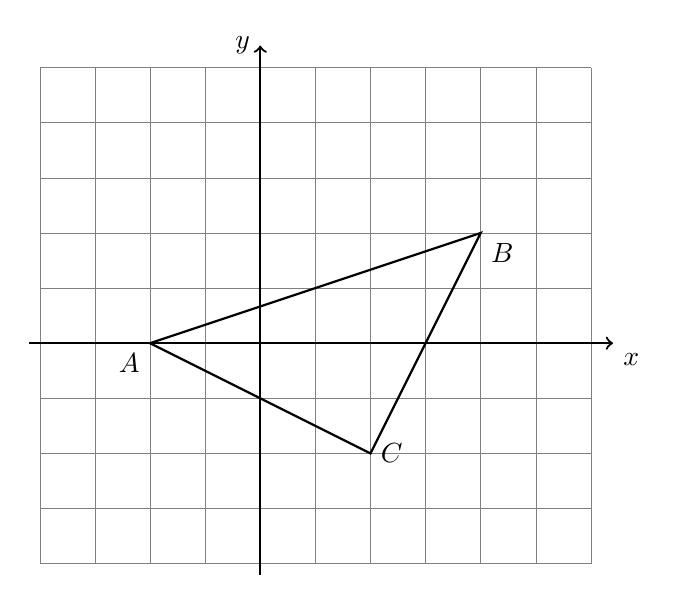
\begin{tikzpicture}[scale=.7]
        \draw [help lines] (-4,-4) grid (6,5);
        \draw [thick, ->] (-4.2,0) -- (6.4,0) node [below right] {$x$};
        \draw [thick, ->] (0,-4.2)--(0,5.4) node [left] {$y$};
        \draw [thick] (-2,0)node[below left]{$A$}--
         (2,-2)node[right]{$C$}--
           (4,2)node[below right]{$B$}--cycle;
      \end{tikzpicture}

      Complete the table of coordinate mappings.\\[0.5cm]
      $A(-2,0) \rightarrow A'(-3,0)$ \vspace{3cm}
    \end{multicols}

\item Given $\triangle USA \sim \triangle MEX$ and $m\angle U =60^\circ$, $m\angle A =85^\circ$. Find the remaining angle measures.
\begin{flushright}
    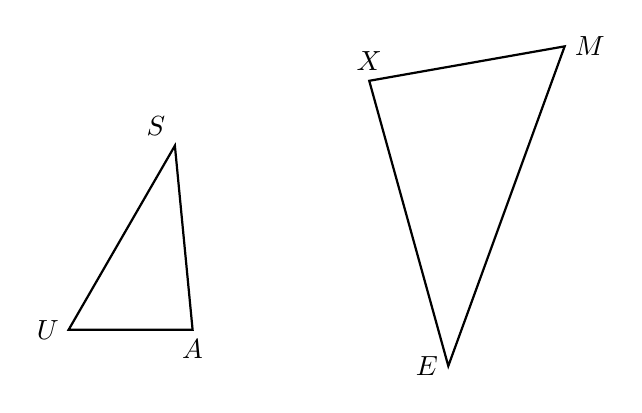
\begin{tikzpicture}[scale=0.9]
    \coordinate [label=above left:$S$](A) at (60:3);
    \coordinate [label=left:$U$](B) at (0, 0);
    \coordinate [label=below:$A$](C) at (0:1.75);
    \draw [thick] (A)--(B)--(C)--cycle;
    \draw [thick, xshift=7cm, yshift=4cm, scale=1.6, rotate=-170] (60:3) node[left]{$E$}--
    (0,0) node[right]{$M$}--
    (0:1.75) node[above]{$X$}--cycle;
  \end{tikzpicture}
\end{flushright}

\newpage
\item A dilation centered at $A$ with a scale factor of $\displaystyle k=1.75$ maps $\triangle ABC \rightarrow \triangle ADE$. Given $AB=12.4$, $AC=8.8$, $DE=13.3$. 
\begin{multicols}{2}
  Find the remaining side lengths.\\[0.25cm]
  $AD=$\\[1cm]
  $AE=$\\[1cm]
  $BC=$\\
  \begin{flushright}
    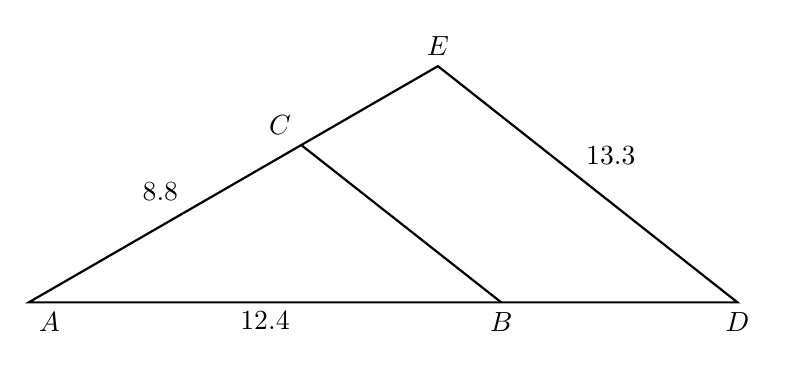
\begin{tikzpicture}[scale=1.2]
      \draw [thick]
      (0,0)node[below right]{$A$}--
      (0:7.5)node[below]{$D$}--
      (30:5)node[above]{$E$}--cycle;
      \draw [thick]
      (0:5)node[below]{$B$}--
      (30:3.33)node[above left]{$C$};
      \node at (0:2.5)[below]{$12.4$};
      \node at (15:6)[right]{$13.3$};
      \node at (35:1.7)[above]{$8.8$};
    \end{tikzpicture}
  \end{flushright}
\end{multicols}\vspace{1cm}

\item Triangle $HTS$, where $H$ = $Home$, is dilated with a scale factor of $k=2$ centered at $H$, yielding $\triangle HLC$, as shown.\\[0.25cm]
Given $HT$ = 8 blocks, $HS$ = 7 blocks, and $LC$ = 18 blocks. There are twenty blocks to a mile.
\begin{enumerate}
  \item Steven walks from school to Tommy's and then walks home. What fraction of a mile did he walk?
\begin{flushright}
  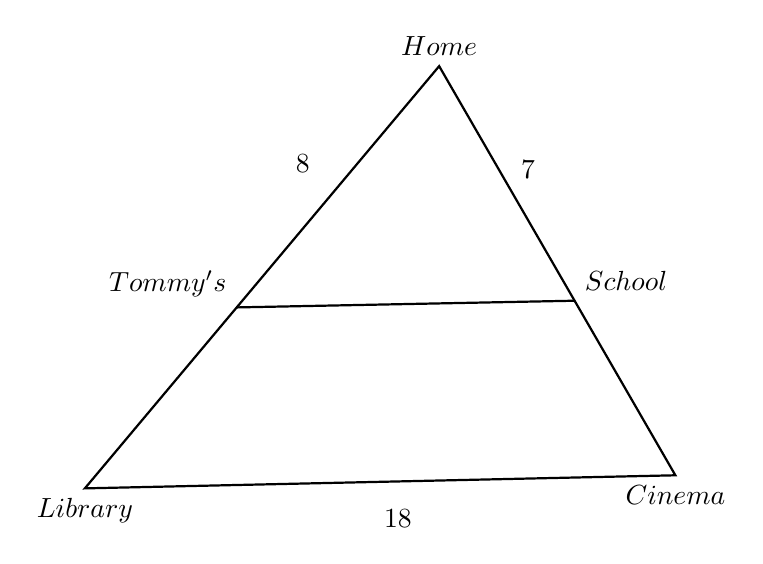
\begin{tikzpicture}[scale=0.8]
    \draw [thick]
    (0,0)node[above]{$Home$}--
    (-130:8.75)node[below]{$Library$}--
    (-60:7.5)node[below]{$Cinema$}--cycle;
    \draw [thick]
    (-130:5)node[above left]{$Tommy's$}--
    (-60:4.3)node[above right]{$School$};
    \node at (-150:2.5)[below]{$8$};
    \node at (-55:2)[right]{$7$};
    \node at (-95:7.5)[above]{$18$};
  \end{tikzpicture}
\end{flushright} 
  \item Steven's sister, Marie, goes to the cinema after school and then walks back home. Did she walk more or less than a mile?
\end{enumerate}

\newpage
\item Show below is a map of Hispanola with a grid of lines of longitude (north south) and latitude (east west). Mark the following features on the map:
\begin{enumerate}
  \item The approximate national border between Haiti and the Dominican Republic at the line of longitude $71.75^\circ$ (through Lago Enriquillo).
  \item The capital city of Santo Domingo at $18.5^\circ$ N, $70^\circ$ W.
  \item The Haitian capital Port-au-Prince at $18.5^\circ$ N, $72.25^\circ$ W.
  \item The world famous Kite Beach, Cabarete at $19.75^\circ$ N, $70.4^\circ$ W.

\begin{flushleft}
  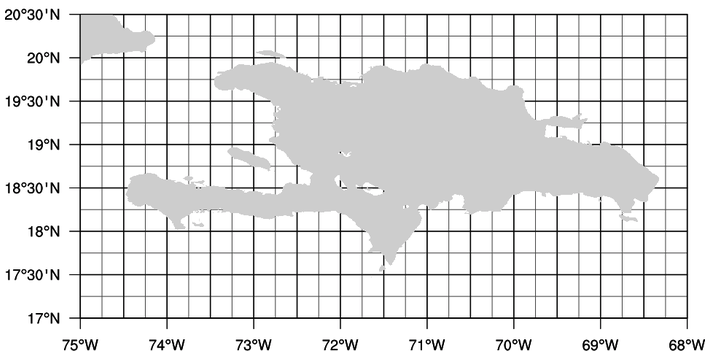
\includegraphics[width=14cm]{DR-map.png}
\end{flushleft}
Each degree of latitude or longitude is approximately 110 kilometers.\\
\item By how many degrees of longitude do Port-au-Prince and Santo Domingo differ?\vspace{1cm}
\item Calculate the distance between the two capital cities.\vspace{2cm}
\item Calculate the distance from Santo Domingo to Cabarete.
\end{enumerate}



\newpage
\item Rotate $\triangle ABC$ $180^\circ$ counterclockwise around the origin. Then, dilate $\triangle A'B'C'$ by a factor of $\displaystyle k=\frac{5}{3}$ centered at the origin to produce $\triangle A''B''C''$. Plot and label the two triangles in the graph below.
\begin{center}
  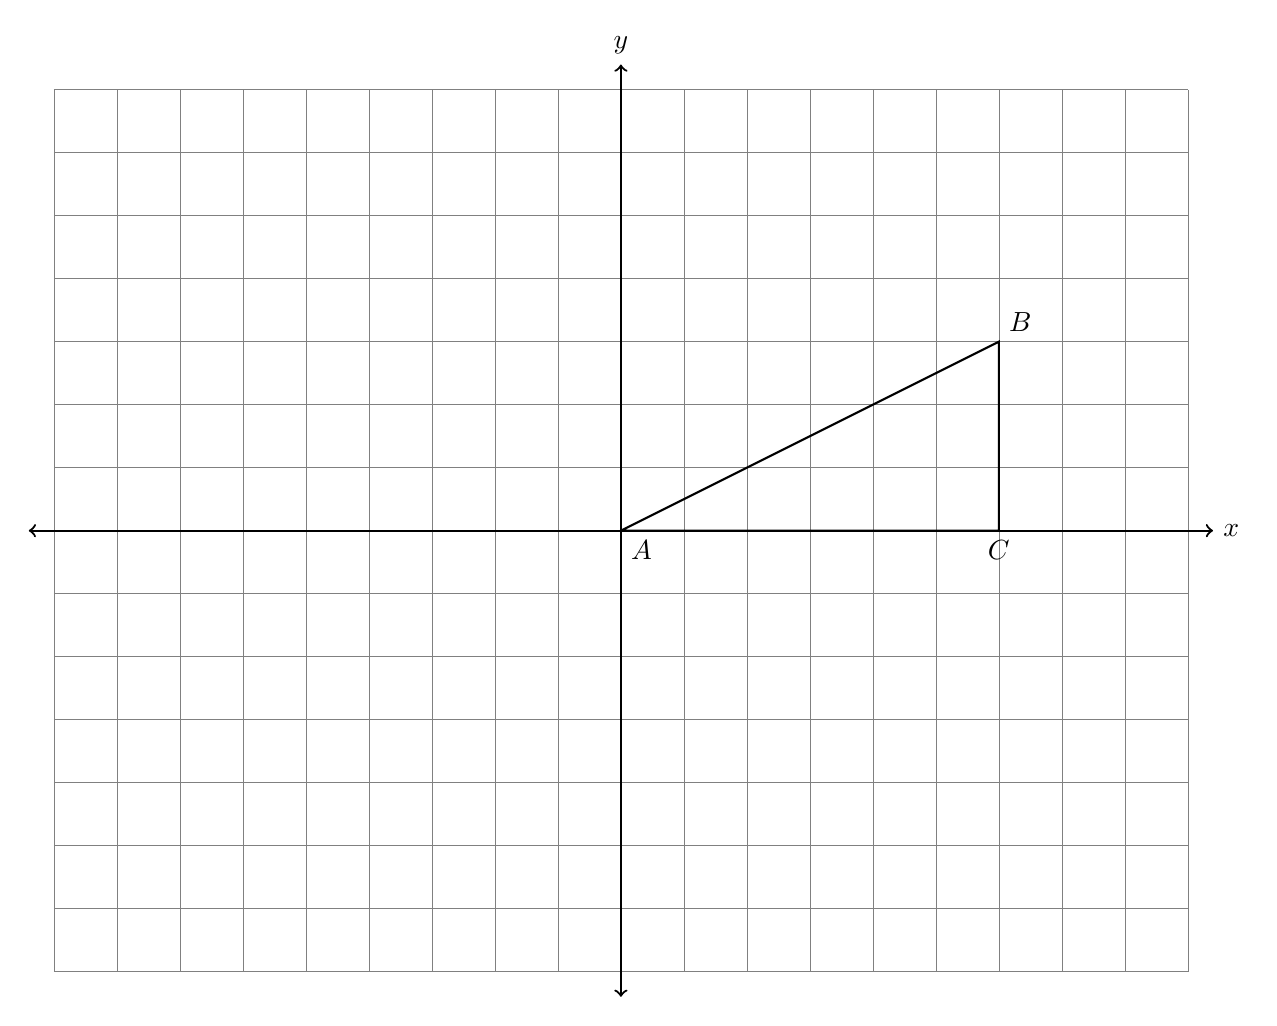
\begin{tikzpicture}[scale=0.8]
    \draw [help lines] (-9,-7) grid (9,7);
    \draw [thick, <->] (-9.4,0) -- (9.4,0) node [right] {$x$};
    \draw [thick, <->] (0,-7.4)--(0,7.4) node [above] {$y$};
    \draw [thick]
      (0,0) node[below right] {$A$}--
      (6,3) node[above right] {$B$}--
      (6,0) node[below] {$C$}--
      cycle;
  \end{tikzpicture}
\end{center}
Would the same triangle result if you dilated first and then rotated? When are rotation and dilation ``commutative'', never, sometimes, always?

\end{enumerate}
\end{document}
